\documentclass[12pt]{article}

\title{A visual method for generating the separating isosurface of two classes of objects in two-dimensional space}
\author{
Shawn Halayka\footnote{Independent -- sjhalayka@gmail.com}
}


\date{\today\;\currenttime}

\usepackage{datetime}
\usepackage{listings}
\usepackage{cite}
\usepackage{xcolor}
\usepackage{graphicx}
\usepackage{setspace}
\usepackage{amsmath}
\usepackage{url}
\usepackage{amsfonts}
\usepackage{caption}
\usepackage{subcaption}

\usepackage[margin=1in]{geometry}

%\doublespace

\begin{document}




\maketitle

\begin{abstract}
With regard to the separating isosurface of two classes of objects in two-dimensional space, the transition from nonlinear to linear is documented.
\end{abstract}




\section{Introduction}

Iron out the wrinkles by downsizing.
Can also convolve the images, like blurring, which can be used to melt away higher-frequency detail.
Balance between high bias and high variance.
Marching Squares works as a radial-based isosurface generator.





\begin{thebibliography}{9}

\bibitem{mc} James, et al. An Introduction to Statistical Learning with Applications in R. ISBN: 978-1-0716-1417-4

\end{thebibliography}






\begin{figure} 
\centering
  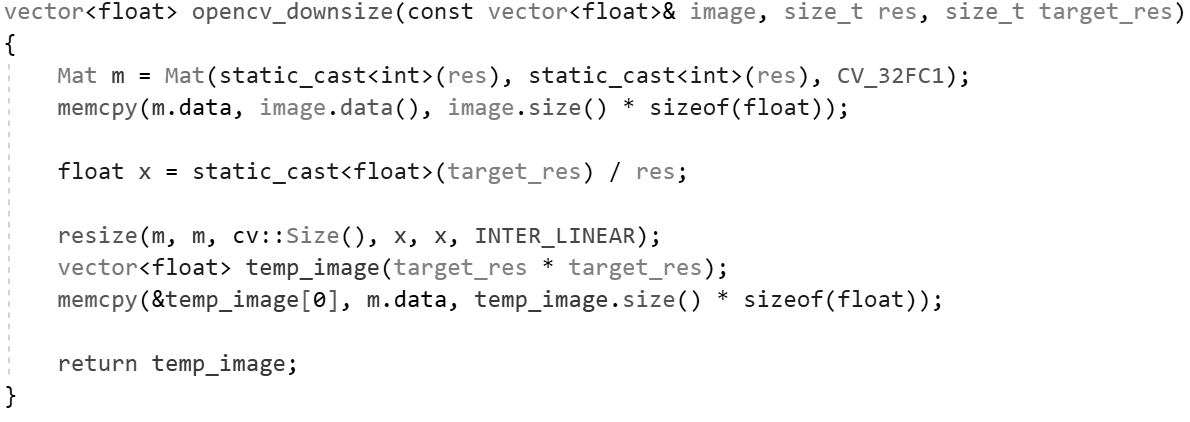
\includegraphics[width = 4 in]{downsize_code.png}
  \caption{Code to downsize an image, using OpenCV.
}
\end{figure}




\begin{figure} 
\centering
  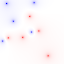
\includegraphics[width = 3 in]{64_res_image.png}
  \caption{Bitmap image used as input to the Marching Squares algorithm. 
Image size is 64x64.
Colour falls of with distance.
}
\end{figure}

\begin{figure} 
\centering
  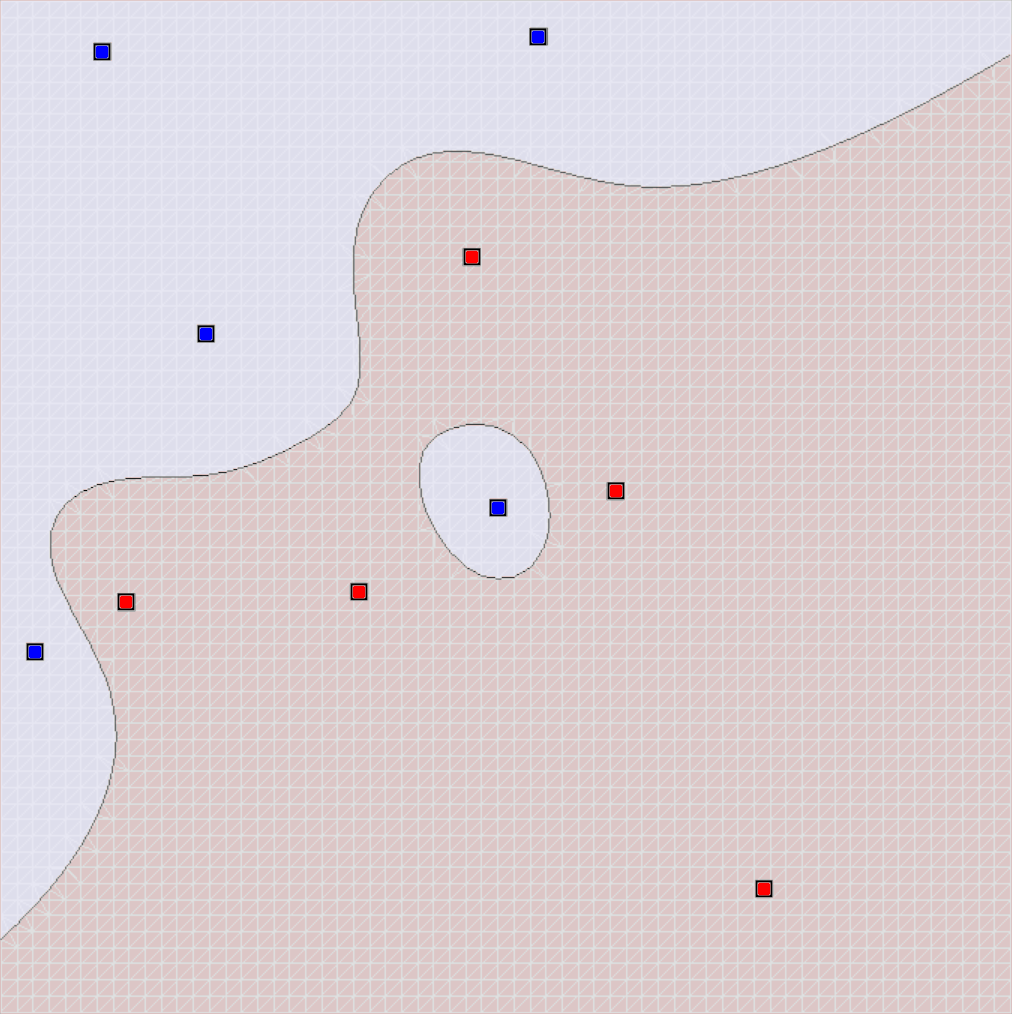
\includegraphics[width = 3 in]{64_res.png}
  \caption{Nonlinear, radial, separation. Grid resolution is 64x64.
}
\end{figure}


\begin{figure} 
\centering
  
\includegraphics[width = 3 in]{16_res_image.png}
  \caption{Bitmap image used as input to the Marching Squares algorithm.
Image size is 16x16.
}
\end{figure}


\begin{figure} 
\centering
  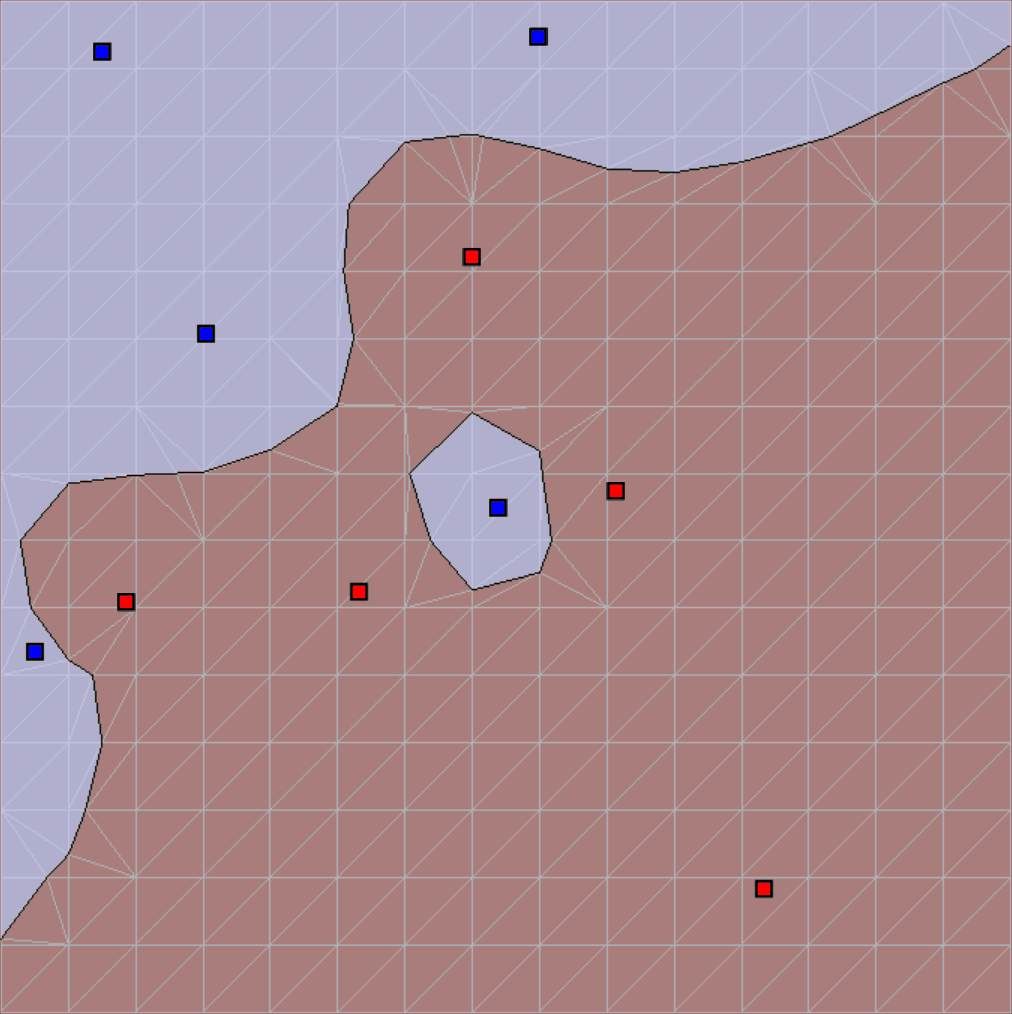
\includegraphics[width = 3 in]{16_res.png}
  \caption{Nonlinear, radial, separation. Grid resolution is 16x16.
}
\end{figure}

\begin{figure} 
\centering
  
\includegraphics[width = 3 in]{2_res_image.png}
  \caption{Bitmap image used as input to the Marching Squares algorithm.
Image size is 2x2.
}
\end{figure}


\begin{figure} 
\centering
  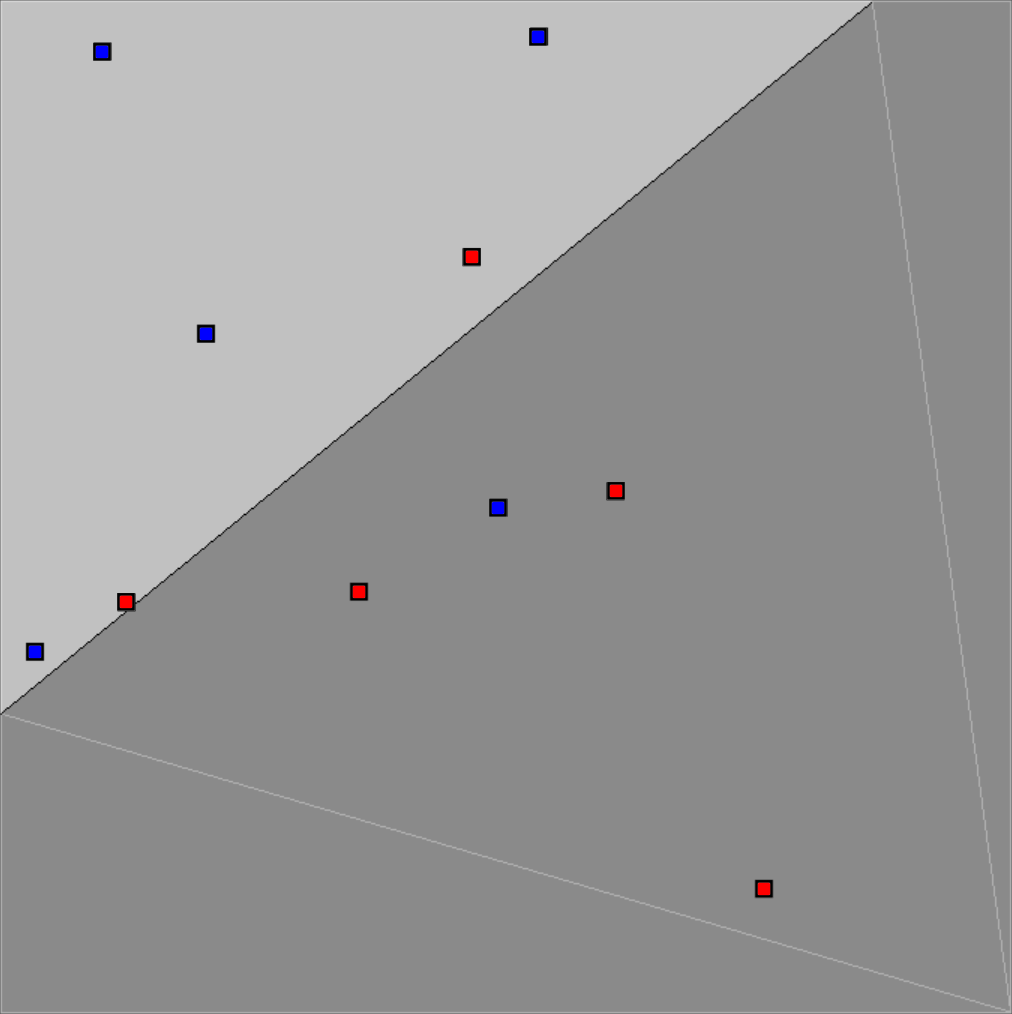
\includegraphics[width = 3 in]{2_res.png}
  \caption{Linear separation. Grid resolution is 2x2.
}
\end{figure}












\end{document}









